\documentclass[12pt]{article}
\usepackage[margin=1in]{geometry}
\usepackage{setspace}
\usepackage{graphicx}
\usepackage{subcaption}
\usepackage{amsmath}
\usepackage{color}
\usepackage{hyperref}
\usepackage{multicol}
\usepackage{framed}
\usepackage{xcolor}
\usepackage{wrapfig}
\usepackage{float}
\usepackage{fancyhdr}
\usepackage{verbatim}
\usepackage{colortbl}
\usepackage{array, booktabs, caption}
\usepackage{makecell}

\pagestyle{fancy}
\lfoot{\textbf{Open Source Rover Mechanical Assembly Manual}}
\rfoot{Page \thepage}
\lhead{\textbf{\leftmark}}
\rhead{\textbf{\rightmark}}
\cfoot{}
\renewcommand{\footrulewidth}{1.8pt}
\renewcommand{\headrulewidth}{1.8pt}
\doublespacing
\setlength{\parindent}{1cm}

% Parts list tables
\renewcommand\theadfont{\bfseries}
\newcolumntype{I}{ >{\centering\arraybackslash} m{2cm} }  % part image
\newcolumntype{N}{ >{\centering\arraybackslash} m{3cm} }  % part name
\newcolumntype{Q}{ >{\centering\arraybackslash} m{0.75cm} }  % ref & qty


\begin{document}

\newcommand\partimg{\includegraphics[width=2cm,height=1.25cm,keepaspectratio]}


\title{Open Source Rover: Head Assembly Instructions}
\author{Authors: Michael Cox, Eric Junkins, Olivia Lofaro}

\makeatletter
\def\@maketitle{
\begin{center}
	\makebox[\textwidth][c]{ \includegraphics[width=0.6\paperwidth]{"Pictures/finala".png}}
	{\Huge \bfseries \sffamily \@title }\\[3ex]
	{\Large \sffamily \@author}\\[3ex]
	\includegraphics[width=.65\linewidth]{"Pictures/JPL logo".png}
\end{center}}
\makeatother

\maketitle

\noindent {\footnotesize Reference herein to any specific commercial product, process, or service by trade name, trademark, manufacturer, or otherwise, does not constitute or imply its endorsement by the United States Government or the Jet Propulsion Laboratory, California Institute of Technology. \textcopyright  2018 California Institute of Technology. Government sponsorship acknowledged.}


% Introduction
\newpage


\tableofcontents

\newpage

\section{3D printing}
There are a few components that need to be 3D printed to make the head assembly. You can find the STL files necessary for these prints in the Mechanical/Head Assembly/3D Printed Parts folder of the repository.

\begin{figure}[H]
	\centering
	\includegraphics[width=0.75\textwidth]{"Pictures/S43".PNG}
	\caption{3D printed Head piece}
\end{figure}


If you do not have a 3D printer there are a number of online 3D printing services available, an example of which can be found at:

\begin{itemize}
	\item \href{https://www.makexyz.com/}{https://www.makexyz.com/}
\end{itemize}


\section{Machining/Fabrication}
\subsection{Cutting the PVC Pipe}


\begin{table}[H]
    \centering
    \arrayrulecolor{lightgray}
    \sffamily\footnotesize
    \captionsetup{font={sf,bf}}
    \caption{Parts/Tools Necessary}
    \begin{tabular}{|N|Q|Q|I|N|Q|Q|I|}
        \hline
        \thead{Item} & \thead{Ref} & \thead{Qty} & \thead{Image} & \thead{Item} & \thead{Ref} & \thead{Qty} & \thead{Image} \\
        \hline
        2" PCV Pipe & S29 & 1 & \partimg{../../../images/components/Structural/S29.png} & Vice or V-Clamps & D8 & & \partimg{../../../images/components/Tools/D8.png} \\ \hline
        HackSaw or Bandsaw & D4 & & \partimg{../../../images/components/Tools/D4.png} & & & & \\ \hline
    \end{tabular}
\end{table}


Take the PVC pipe \textbf{S29} (this will be the "neck" of the rover) and cut it to your desired length. For reference, we cut our "neck" PVC pipe to be roughly 6 inches long.


\section{Mechanical Assembly}

\begin{table}[H]
    \centering
    \arrayrulecolor{lightgray}
    \sffamily\footnotesize
    \captionsetup{font={sf,bf}}
    \caption{Parts/Tools Necessary}
    \begin{tabular}{|N|Q|Q|I|N|Q|Q|I|}
        \hline
        \thead{Item} & \thead{Ref} & \thead{Qty} & \thead{Image} & \thead{Item} & \thead{Ref} & \thead{Qty} & \thead{Image} \\
        \hline
        3D Printed Head & S43 & 1 & \partimg{../../../images/components/Structural/S43.png} & \#6-32x3/8" Button Head Screw & B2 & 4 & \partimg{../../../images/components/Screws/B2.png} \\ \hline
        LED Matrix & E37 & 1 & \partimg{../../../images/components/Electronics/E37.png} & \#4-40x1/4" Button Head Screw & B8 & 12 & \partimg{../../../images/components/Screws/B8.png} \\ \hline
        Bore Clamping Hub for 1" PVC & S24 & 1 & \partimg{../../../images/components/Structural/S24.jpg} & M2.5 x 6mm  & B10 & 8 & \partimg{../../../images/components/Screws/B10.png} \\ \hline
        PVC Pipe (Modified) & S29A & 1 & \partimg{../../../images/components/Structural/S29.png} & Arduino Sheild & E2 & 1 & \partimg{../../../images/components/Electronics/E2.png} \\ \hline
	M3 x 6mm Socket Head Cap screw & B14 & 6 & \partimg{../../../images/components/Screws/B14.png} & Laser Cut Arduino Plate & S44 & 1 & \partimg{../../../images/components/Structural/S44.png} \\ \hline
	Laser Cut Head Back Panel & S42 & 1 & \partimg{../../../images/components/Structural/S42.png} & Arduino Uno & E24 & 1 & \partimg{../../../images/components/Electronics/E24.png} \\ \hline 
	M2.5 x 10mm & T10 & 4 & \partimg{../../../images/components/Standoffs/T10.png} & \#4-40 Heat Set Insert & I1 & 8 & \partimg{../../../images/components/Inserts/I1.png}  \\ \hline
    \end{tabular}
\end{table}

\begin{enumerate}

\item \textbf{Assemble the Arduino Stack:} Begin by stacking together the Arduino Uno \textbf{E24}, Arduino Sheild \textbf{E2}, Standoffs \textbf{T10}, Screws \textbf{B10}, and Arduino Plate \textbf{S44} and assemble them in the following stack. 

\begin{figure}[H]
	\centering
  	\begin{minipage}[b]{0.45\textwidth}
		\includegraphics[width=\textwidth]{"Pictures/step-1a".PNG}
  	\end{minipage}
  	\hfill
  	\begin{minipage}[b]{0.45\textwidth}
    		\includegraphics[width=\textwidth]{"Pictures/step-1b".png}
  	\end{minipage}
  	\caption{Building Arduino Stack}
\end{figure}


\item \textbf{Inserting the Heat set inserts:} Insert the \# 4-40 Heat Set Inserts \textbf{I1} into the 3D printed head using a Solder Iron at 460 degrees F, in the locations shown in the following images.

\begin{figure}[H]
	\centering
  	\begin{minipage}[b]{0.45\textwidth}
		\includegraphics[width=\textwidth]{"Pictures/step-2a".PNG}
  	\end{minipage}
  	\hfill
  	\begin{minipage}[b]{0.45\textwidth}
    		\includegraphics[width=\textwidth]{"Pictures/step-2b".png}
  	\end{minipage}
  	\caption{Back panel Inserts}
\end{figure}

\begin{figure}[H]
	\centering
  	\begin{minipage}[b]{0.45\textwidth}
		\includegraphics[width=\textwidth]{"Pictures/step-3a".PNG}
  	\end{minipage}
  	\hfill
  	\begin{minipage}[b]{0.45\textwidth}
    		\includegraphics[width=\textwidth]{"Pictures/step-3b".png}
  	\end{minipage}
  	\caption{Arduino Inserts}
\end{figure}

\item \textbf{Mount the PVC clamping hub:} Using screws \textbf{B2} and attach the PVC clamping hub to the bottom of the 3D printed Head. 

\begin{figure}[H]
	\centering
  	\begin{minipage}[b]{0.45\textwidth}
		\includegraphics[width=\textwidth]{"Pictures/step-4a".PNG}
  	\end{minipage}
  	\hfill
  	\begin{minipage}[b]{0.45\textwidth}
    		\includegraphics[width=\textwidth]{"Pictures/step-4b".png}
  	\end{minipage}
  	\caption{PVC Clamping hub Mount}
\end{figure}

\item \textbf{Attach PVC Pipe:} Slot the PVC pipe \textbf{S29} into the clamping hub and then tighten down the screws on the clamping hub

\begin{figure}[H]
\centering
  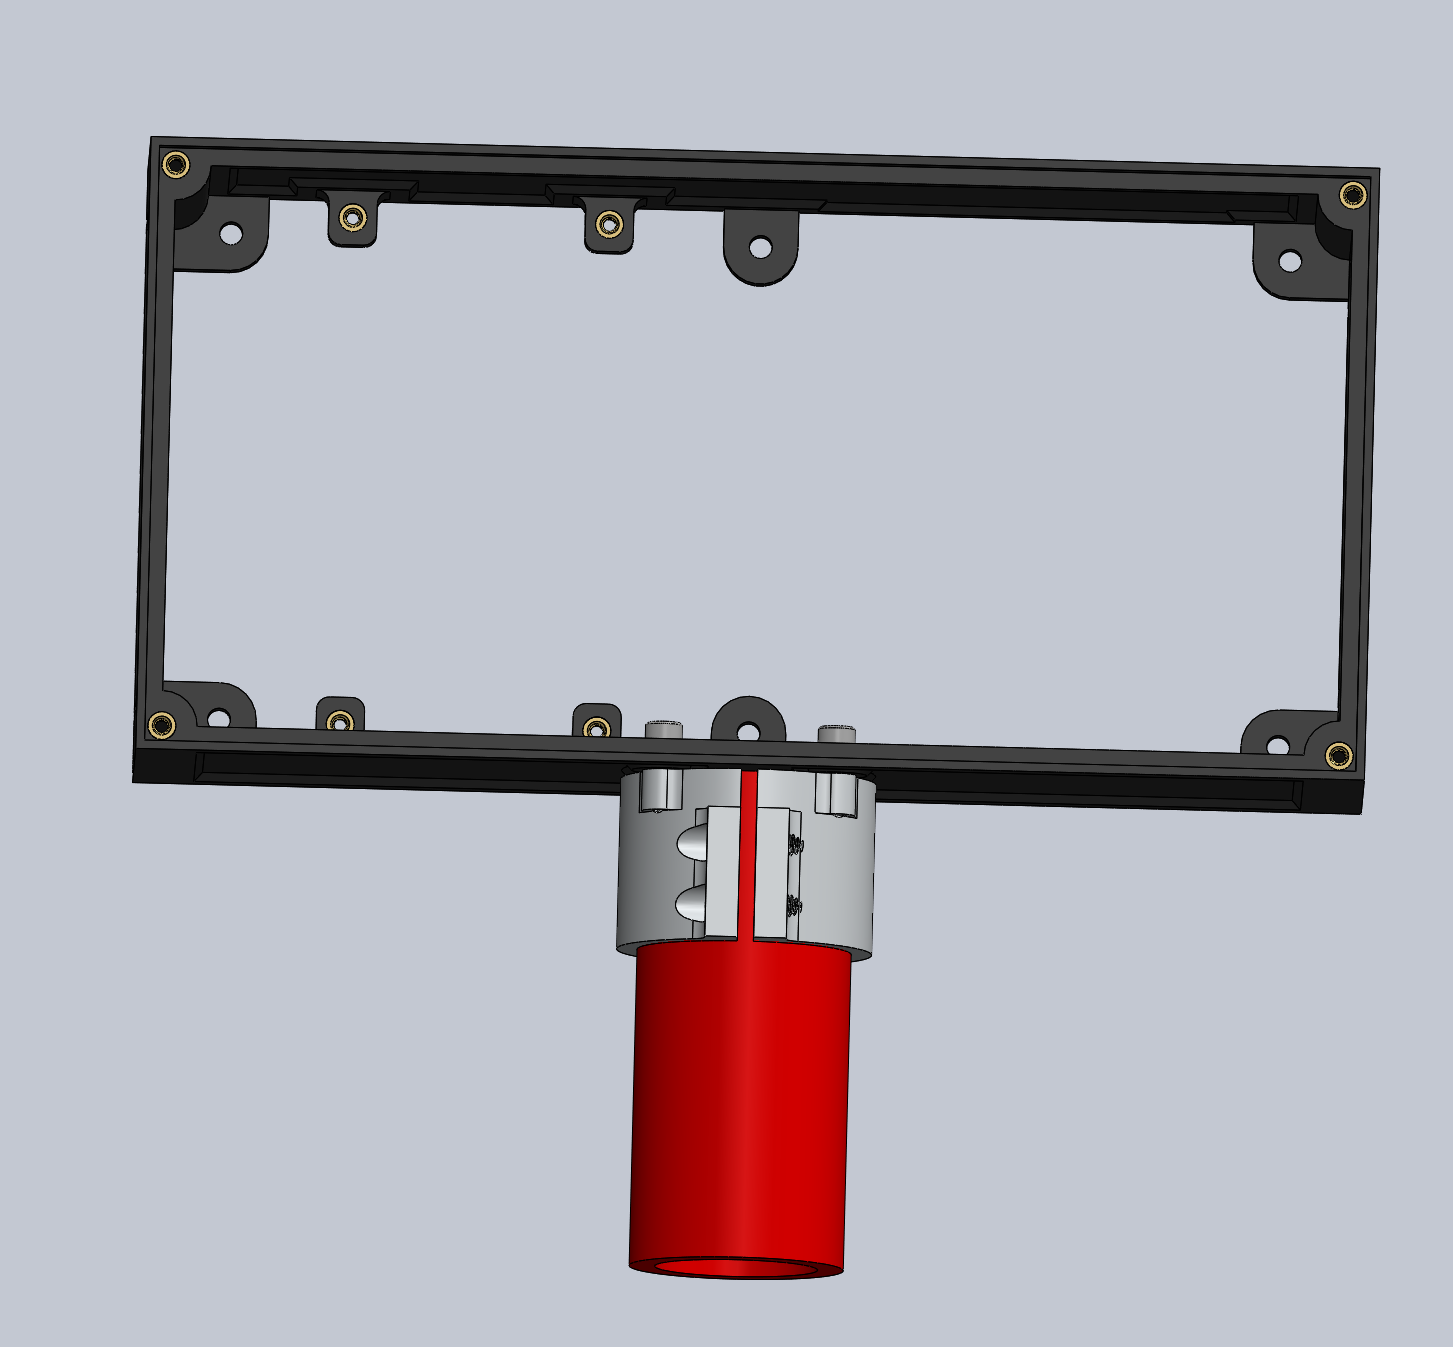
\includegraphics[width=0.8\linewidth]{"Pictures/step-5a.png}
	\caption{Neck Attachment}
\end{figure}

\item \textbf{Attaching the LED Matrix} Using Screws \textbf{B14} attach the LED Matrix \textbf{E37} to the front of the Head assembly. 

\begin{figure}[H]
	\centering
  	\begin{minipage}[b]{0.45\textwidth}
		\includegraphics[width=\textwidth]{"Pictures/step-6a".PNG}
  	\end{minipage}
  	\hfill
  	\begin{minipage}[b]{0.45\textwidth}
    		\includegraphics[width=\textwidth]{"Pictures/step-6b".png}
  	\end{minipage}
  	\caption{LED Matrix Attachment}
\end{figure}

\item \textbf{Mount the Arduino Inside:} Take the Arduino Plate assembly and mount it using screws \textbf{B8} to the Heat set inserts on the posts inside the head

\begin{figure}[H]
	\centering
  	\begin{minipage}[b]{0.45\textwidth}
		\includegraphics[width=\textwidth]{"Pictures/step-7a".PNG}
  	\end{minipage}
  	\hfill
  	\begin{minipage}[b]{0.45\textwidth}
    		\includegraphics[width=\textwidth]{"Pictures/step-7b".png}
  	\end{minipage}
  	\caption{Arduino Plate Integration}
\end{figure}

\item \textbf{Back Plate Attachment:} Attach the Laser Cut Back plate \textbf{S42} onto the back of the head assembly using screws \textbf{B12}.

\begin{figure}[H]
	\centering
  	\begin{minipage}[b]{0.45\textwidth}
		\includegraphics[width=\textwidth]{"Pictures/step-8a".PNG}
  	\end{minipage}
  	\hfill
  	\begin{minipage}[b]{0.45\textwidth}
    		\includegraphics[width=\textwidth]{"Pictures/step-8b".png}
  	\end{minipage}
  	\caption{Back Panel Assembly}
\end{figure}


The Head is now finished!

\begin{figure}[H]
	\centering
  	\begin{minipage}[b]{0.45\textwidth}
		\includegraphics[width=\textwidth]{"Pictures/finala".PNG}
  	\end{minipage}
  	\hfill
  	\begin{minipage}[b]{0.45\textwidth}
    		\includegraphics[width=\textwidth]{"Pictures/finalb".png}
  	\end{minipage}
  	\caption{Finished Head Assembly}
\end{figure}

\end{enumerate}

\end{document}
